% !Mode:: "TeX:UTF-8"

\chapter{分布式轨迹语义表征}
\label{chapter:main2}

要在轨迹上进行信息挖掘,首先需要在轨迹上定义一个空间,使得轨迹中蕴含的语义可以得到表示,同时使不同轨迹之间感兴趣的相似度能够得到衡量。在不同的场景下,研究者们纷纷提出利于自己算法运行的轨迹表征方法,然而根据应用定下的表征通常没有普适性。为此,本文提出了一种鲁班的轨迹表征方法,使得各种感兴趣的语义都能根据需求融入此表征方法中,进而为后续轨迹挖掘任务打下基础。


\section{问题描述}
如上文所述,传统的轨迹挖掘算法汇总,轨迹通常有三种表征方式:基于采样点的表征、基于线段的表征以及基于特征的表征。然而这三种表征方式在现在的挖掘需求中都有不足:主要关注地理信息,几乎没有考虑具体的语义知识。因此,在表征上建立的索引系统将给后续挖掘任务带来很多限制。

为了衡量语义相似性,应该为轨迹数据创造一种新的表征,并在这种表征上定义新的轨迹相似性度量标准。举一个例子,图\ref{fig:introduction}(a)显示了葡萄牙波尔图的三个出租车轨迹(即$ T_1, T_2$和$T_3 $)。 如果我们只考虑三个轨迹的几何属性,$ T_1 $和$ T_2 $之间的相似性高于$ T_2 $和$ T_3 $之间的相似性。但是,通过考虑城市的交通系统(即结构信息)和区域功能(即领域知识), 由于这两条轨迹都表明了从农村地区到市中心的高速公路运输,而$T_1$意味着从机场到海滨地区的国家公路,则可以得出$ T_2 $更类似于$ T_3 $的结论(图\ref{fig:introduction}(b))。

在本章中,在上一章节\Cascade算法的输出的多层次ROI网络的基础上,我们利用网络的拓普信息、轨迹的时间信息以及其他的领域知识,用一个层次嵌入模型将ROI网络上的节点嵌入到一个隐空间中,使之有定长的表征。这个过程展现在图\ref{fig:introduction}(c)中。在该表征基础上,语义检索任务可以被铸造为通过简单地计算两个向量之间的欧几里德距离来搜索最相似的向量到目标向量的问题。

\tabcolsep=0.5pt
\begin{figure}[!htb]
\centering
\begin{tabular}{cc}
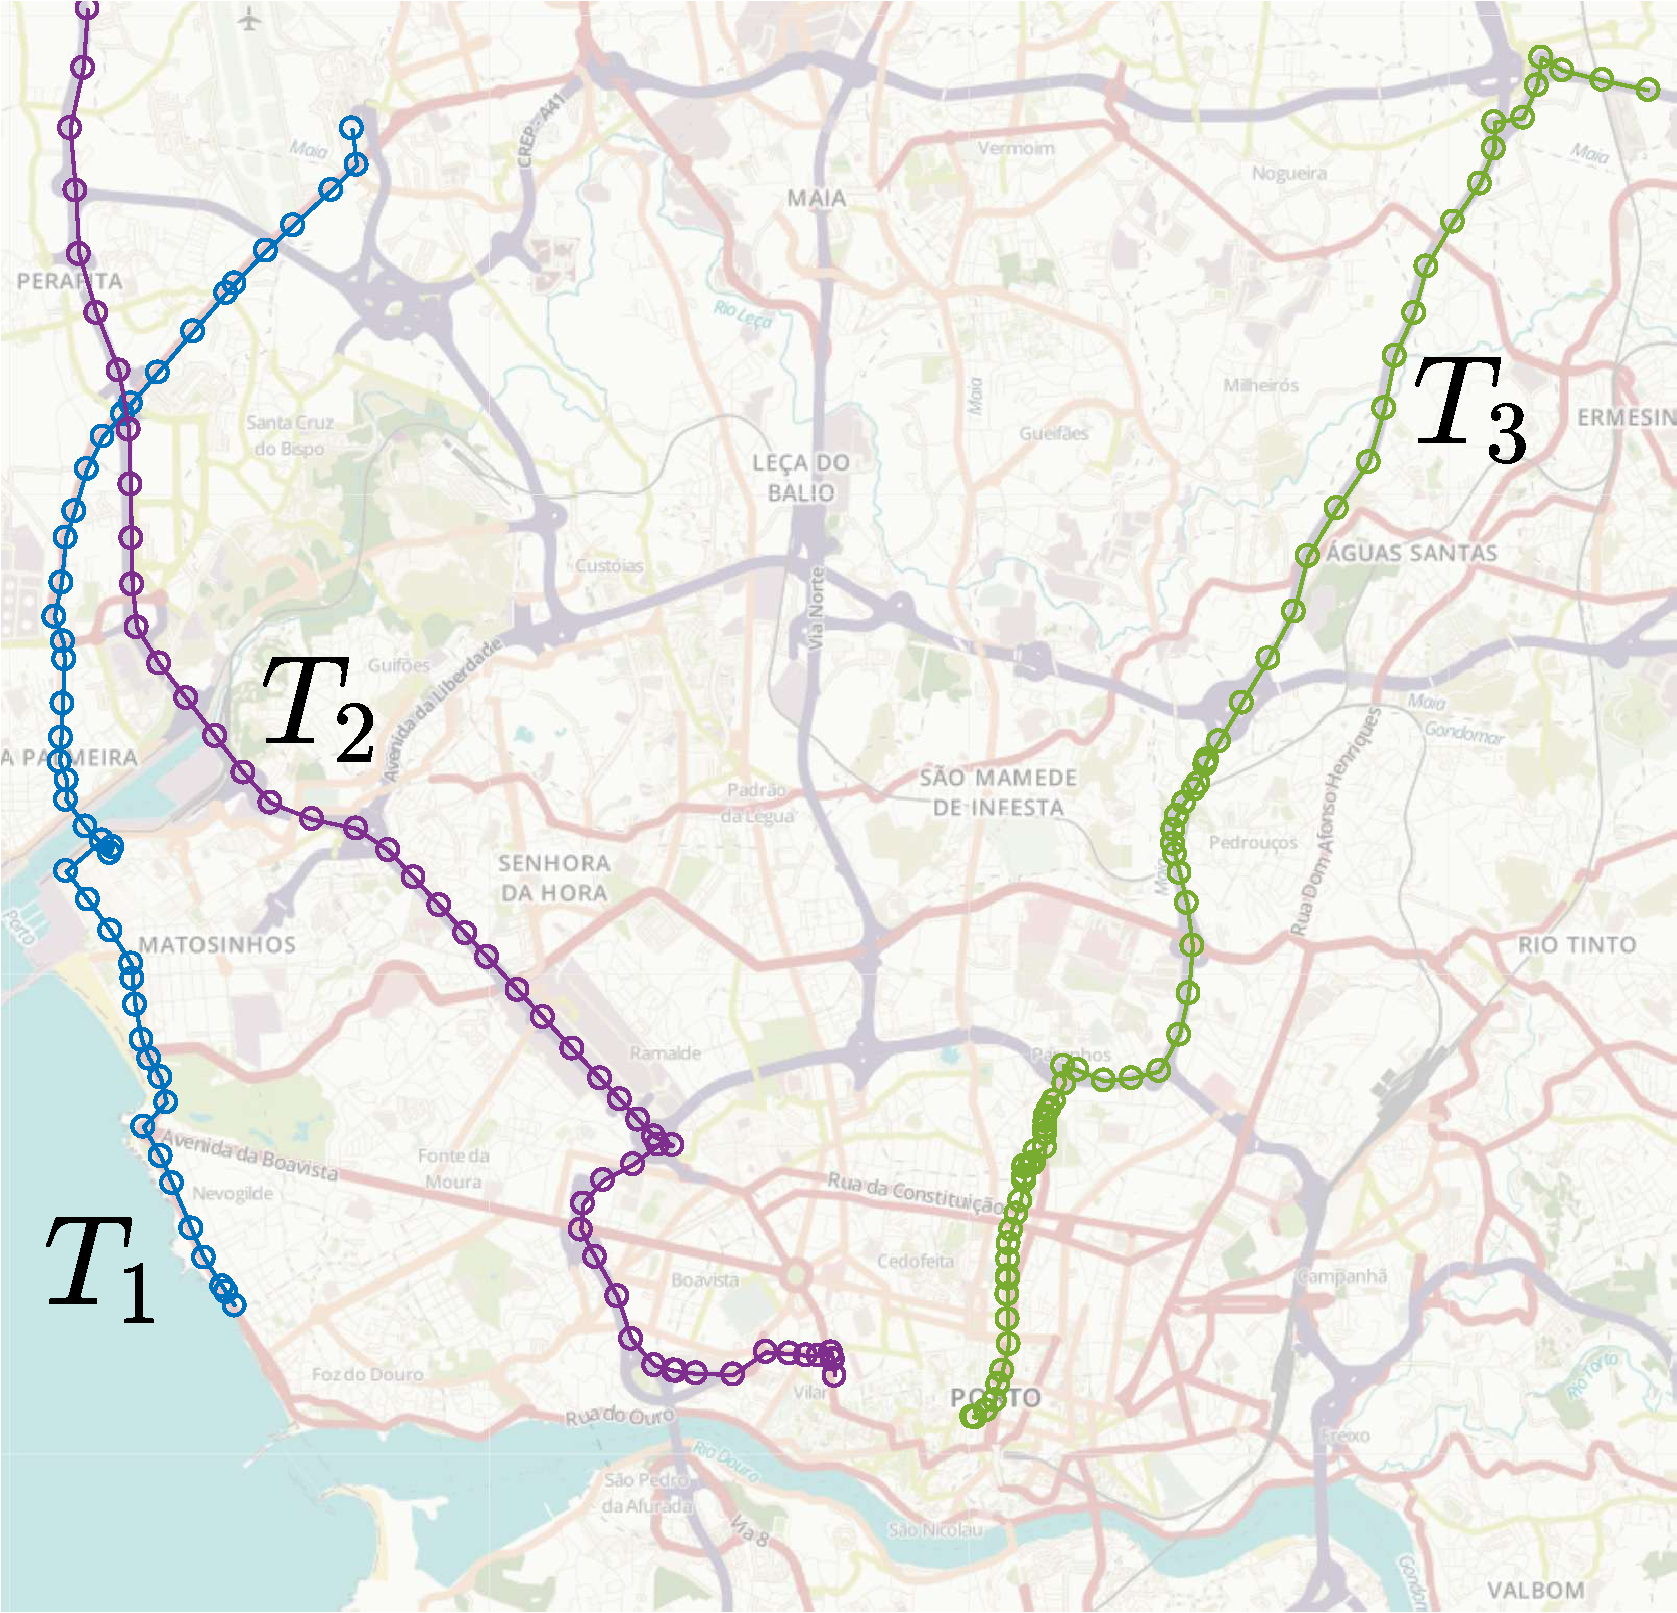
\includegraphics[width=50mm]{pics/introduction1.pdf} & 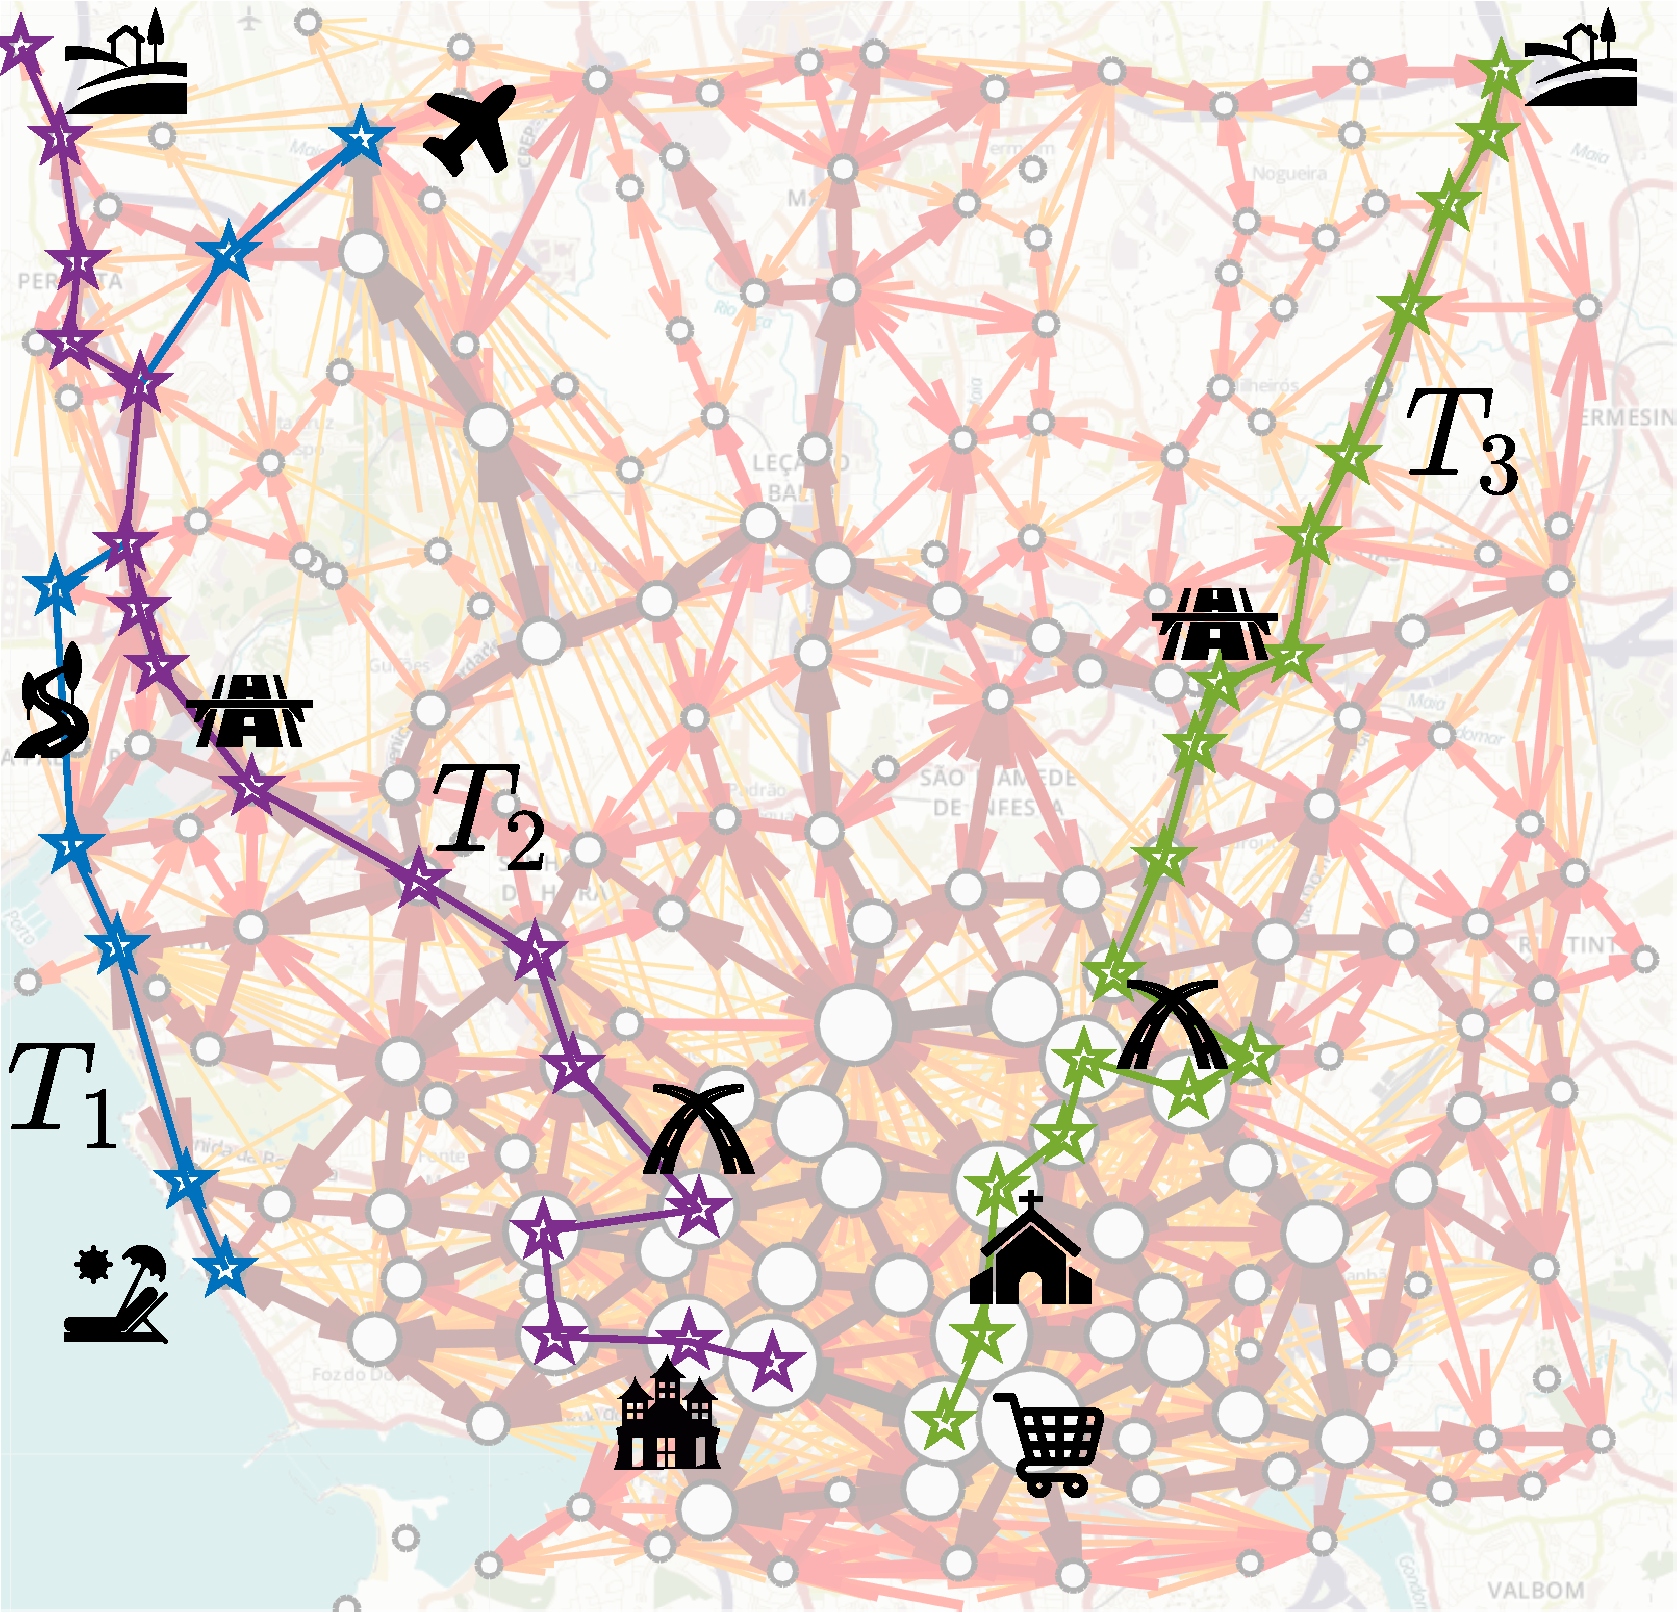
\includegraphics[width=50mm]{pics/introduction2_w.pdf}\\
\multicolumn{2}{c}{\includegraphics[width=100mm]{pics/introduction.pdf}}
\end{tabular}
% \vspace{-2mm}
\caption {轨迹分布式语义表征示意图。(a)葡萄牙波尔图市的三条出租车轨迹;(b) 三条轨迹被\Cascade转换为了ROI序列的表示;(c)将地理序列表示转换为分布式向量表征。}
% \vspace{-3mm}
\label{fig:introduction}
\end{figure}


\section{ROI网络上分布式ROI与轨迹语义嵌入模型}
在上一章的\Cascade算法作用在轨迹数据集上,提取出分层ROI网络之后,每条轨迹将被表征为网络的每个层上的ROI序列。受自然语言处理(NLP)中的词嵌入方案的启发,我们提出了一种嵌入模型,用于进一步将ROI和轨迹转换为语义空间中的连续向量,从而揭示轨迹数据中隐藏的语义信息。

\subsection{单层语义ROI嵌入模型}
嵌入模型的关键是选择给定对象的邻域或上下文,以便可以获得对象之间的关系或者相似度。因此,我们从两个方面考虑ROI的嵌入邻居:几何邻居和语义邻居。

\smallsection{几何邻居}
给定一个ROI,其几何邻居是围绕该ROI的在ROI网络被轨迹以$W$跳能连接起来的其他ROI。 图\ref{fig:context}用$W =2$的几何邻居来作为展示,被绘作绿色和蓝色圆圈。例如,${ROI}_k $是$ {ROI} _i $的几何邻域之一。

\smallsection{语义邻居}
由于ROI不仅仅是网络上的节点,它还代表了一个富含各种语义信息的区域。 为了对丰富的语义进行编码,我们从以下角度定义给定ROI的语义邻域:

\tabcolsep=1pt
\begin{figure*}[!t]
\centering
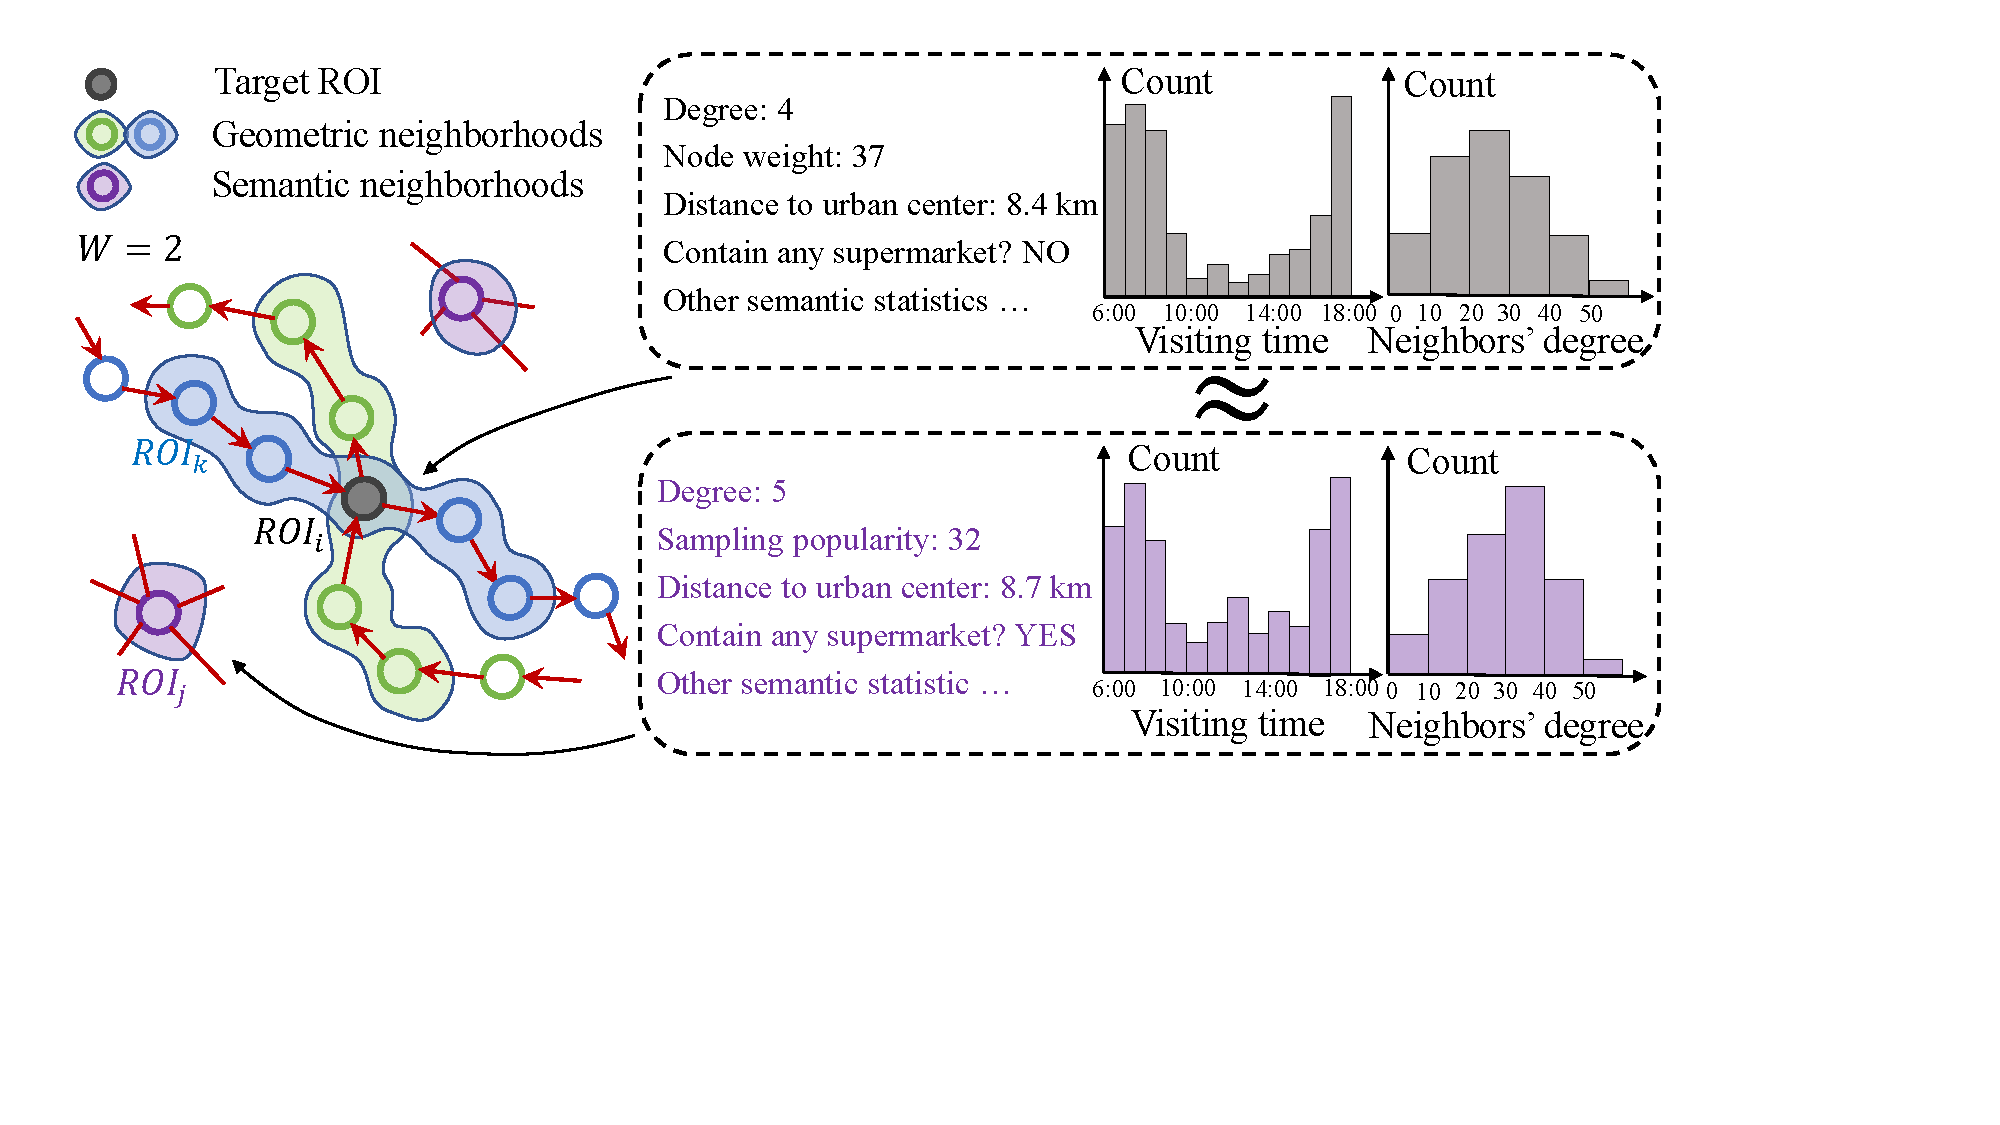
\includegraphics[width=130mm]{pics/embedding.pdf}
\caption {ROI两种邻居示意图。}
% \vspace{-4mm}
\label{fig:context}
\end{figure*}

\begin{itemize}
\item \textbf{网络拓扑属性。} 多层次ROI网络是轨迹数据的一种紧凑表示,从中可以提取城市交通网络的结构状况的统计信息。 具体地,ROI的节点权重是该ROI节点表示GPS点的数目,可以反映该区域的人口密度。ROI网络的边表示两个区域之间的运输流量的强度。ROI的节点度信息反映了这个地区是否是城市的枢纽区域。邻居ROI的度分布可以从更高的层次反映出该地区的重要性和连续性。 例如,如果两个ROI在上述方面彼此相似,则它们可能分别代表一个枢纽巴士站和一个中心火车站,或一个大的公司和一个大学校园。

\item \textbf{时间上下文。}应用\CascadeSync算法后,ROI网络中也会保留时间信息。访问时间和停留时间的分布可以反映一个地区的时间模式。例如,一个地区包含许多餐馆,则访问它们的轨迹主要集中在午餐时间和晚餐时间。而住宅区的也具有鲜明的特征,因为大多采样点在整个晚上都在这儿静止。

\item \textbf{领域知识。}与网络属性和时间信息不同,领域知识不能从轨迹数据中提取。相反,领域知识是将嵌入模型作为一种监督的辅助信息。例如,一个ROI与城市中心点之间的距离,或者一个ROI是否代表道路交叉点,超市或危险犯罪区域等。
\end{itemize}




图\ref{fig:context}给出了ROI邻居的示意图,其中紫色圆圈代表的${ROI}_j$是目标${ROI}_i$的一个语义邻居。虽然它们在网络上的跳数超过了$W=2$跳,但明显${ROI}_j$的语义信息与${ROI}_i$的相似度比其他ROI要大。

一旦获得几何和语义邻域,我们就可以将ROI嵌入到高维空间中,这一步借用了带有负抽样(SGNS)架构的思想\citeup{mikolov2013distributed}。

\smallsection{嵌入模型}给定一个轨迹数据集$\mathcal{T}$,在ROI网络上的任意一层,假设$w$是一个该层的ROI,$N(w)$是$w$两种类型邻居的集合,$NEG(w)$表示$w$的负样本集合。则定义从任意$u\in{N(w)}$转移到任意一个目标ROI$v$的概率如下:
\begin{equation}
\label{eq:transP}
p(v|u) =
\begin{cases}
\sigma(\vec{t_w}\cdot{}\vec{s_u}) & \text{if } v = w,\\
1- \sigma(\vec{t_v}\cdot{}\vec{s_u}) & \text{otherwise}.
\end{cases}
\end{equation}
其中$\sigma(x)=1/(1+\exp{(-x)})$是sigmoid函数。$\vec{s_u}$与$\vec{t_v}$是ROI$u$和$v$的嵌入向量。


\begin{figure*}[!t]
\centering
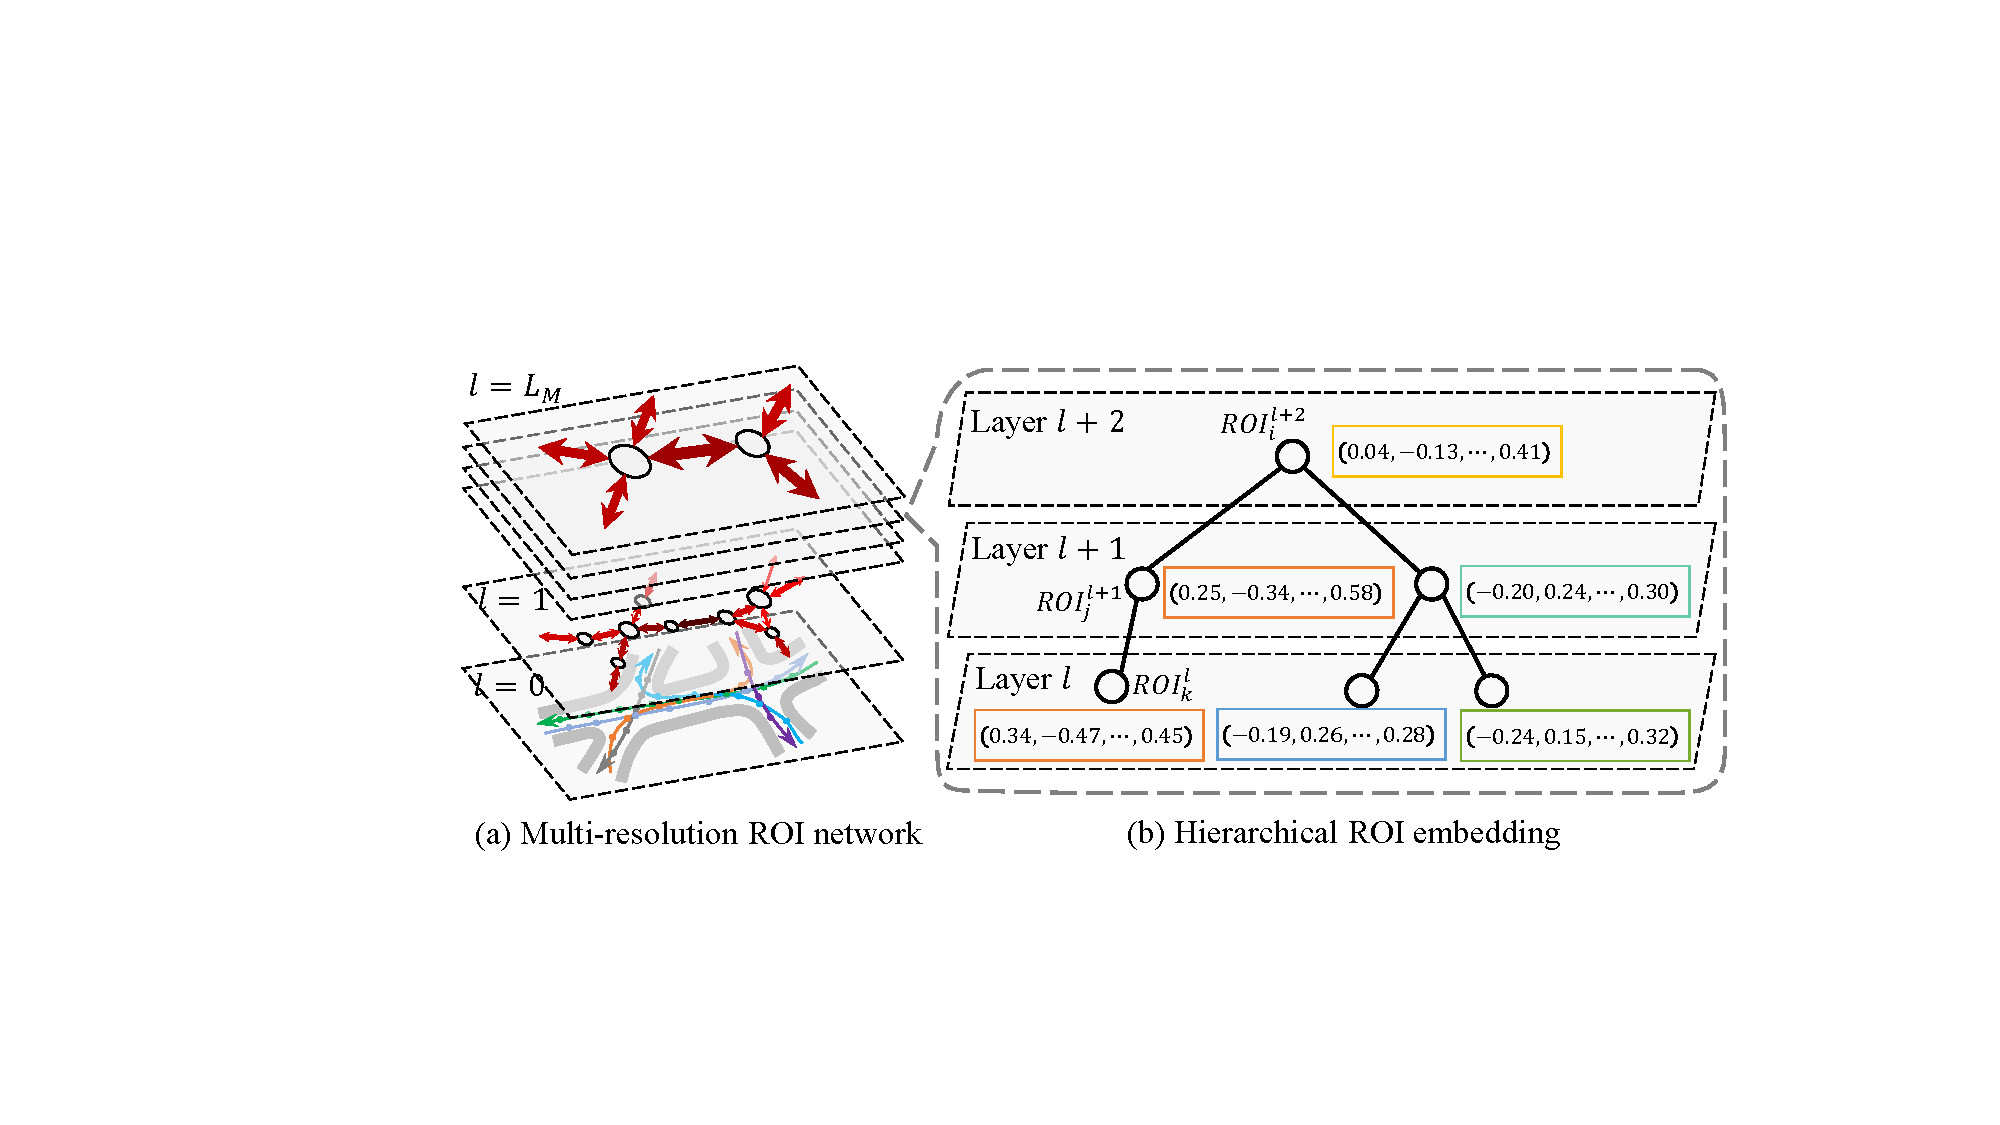
\includegraphics[width=130mm]{pics/Hembedding.pdf}
\caption {多层次语义ROI网络上的嵌入表征示意图。}
\label{fig:Hembedding}
\end{figure*}

模型的最大似然函数可写为:
\begin{equation}
\label{eq:optimizeFun}
L_{H^l} = \log\prod_{w\in{\mathcal{ROI}}^l}\prod_{u \in N(w)}{\hspace{-2mm}\sigma(\vec{t_w}\cdot{}\vec{s_u})}\hspace{-4mm}\prod_{v \in NEG(w)}{\hspace{-4mm}[1-\sigma(\vec{t_v}\cdot{}\vec{s_u})]}
\end{equation}
\begin{displaymath}
\hspace{2mm}= \hspace{-1mm}\sum_{\hspace{-2mm}w\in{\mathcal{ROI}}^l}\hspace{-2mm}\sum_{\hspace{2mm}u \in N(w)}\hspace{-1mm}\left\{{\hspace{-1mm}}\log\sigma(\vec{t_w}\cdot{}\vec{s_u})+ \hspace{-4mm}\sum_{v \in NEG(w)}{\hspace{-3mm}\log[1-\sigma(\vec{t_v}\cdot{}\vec{s_u})]}\right\}, \nonumber
\end{displaymath}

这个似然函数在嵌入空间中表示目标ROI的向量应该尽可能接近其邻域的所有矢量,同时区别其负样本的向量。

% \subsection{时间复杂度分析}
ROI嵌入模型的时间复杂度为$O(K \times N\times N_1\times N_2)$,其中$N$是点的数目,$N_1$是两种邻居的平均数量,$N_2$是负采样的样本个数,$K$是迭代的次数。

\subsection{多层次语义ROI网络的嵌入模型}

\smallsection{多层ROI网络不同层间的信息扩散}
嵌入过程在分层ROI网络的每一层上进行。此外,考虑到每个ROI都有父节点或子节点(除非它位于顶层或底层),我们做出一个直观的假设:每个ROI应该尽可能地在嵌入空间里与其父节点接近(如果存在)。 这种假设在显示中的语义下是合理的。例如,一个大商区的语义含义应包含位于该地区的公司或商店提供的所有功能。我们将这种信息传播写入嵌入模型的正则化项中:
\begin{equation}
\label{eq:optimizeFun2}
L_{V^l} = \sum_{w\in{\mathcal{ROI}^l}}\frac{1}{2}||\vec{t_w}-\vec{t_{\pi(w)}}||^2_2 + \frac{1}{2}||\vec{s_w}-\vec{s_{\pi(w)}}||^2_2,
\end{equation}
其中$\pi(w)$是ROI$w$的父节点。事实上父子节点间的影响可由在他们各自的向量上的约束来表示。图\ref{fig:Hembedding}(b)给出了一个例子,其中${ROI}_j^{l+1}$是第$l+1$层的一个ROI,它的向量被其父节点${ROI}_i^{l+2}$的向量和其子节点的${ROI}_k^{l}$的向量所约束。



最后,我们将原始的嵌入模型(\ref{eq:optimizeFun})以及约束项(\ref{eq:optimizeFun2})结合起来,得到了最后的目标方程:
\begin{equation}
\label{eq:optimizeFunAll}
\max \sum_{l=1:L_M} L_{H^l} - \alpha\hspace{-2mm}\sum_{l=1:L_M-1}\hspace{-2mm}L_{V^l}
\end{equation}
其中$\alpha$是一个折中系数。上面这个优化式可由随机梯度下降法(Stochastic Gradient Descent, SGD)来进行优化求解。参数的梯度项写在了算法\ref{alg:embedding}的7-17行里。



\subsection{轨迹的语义嵌入模型。}
当我们得到所有ROI的嵌入向量后,我们可用ROI的权值加权求和得到轨迹的嵌入向量。给定一条轨迹$T^l = \{{ROI}^l_1, {ROI}^l_2, \cdots, {ROI}^l_n\}$在第$l$层上的表示。轨迹$T$最终的嵌入向量$\text{vec}(T)$可以表示为:
\begin{equation}
\label{eq:traVector}
\text{vec}(T) = \sum_{l=1}^{L_M}\sum_{i=1}^n\tau^l_i\cdot\text{vec}({ROI}^l_i),
\end{equation}
其中$\tau_i^l$是${ROI}^l_i$的权值,代表了轨迹$T$停留在${ROI}^l_i$的时间。注意这里也可以用更复杂的测量来求的轨迹的嵌入向量,比如加入衰减函数等。

值得注意的是,虽然这种获得轨迹向量的方式比起其他复杂的方法\citeup{socher2011dynamic,kalchbrenner2014convolutional,tai2015improved}要简单得多,但是简单的加权模型也非常的有效\citeup{blacoe2012comparison}。Wieting等人 \citeup{wieting2015towards}甚至证明了简单的加权模型性能要比复杂的神经网络要更好。再者,简单加权也是符合常识的:轨迹总是由采样点构成的。


\begin{algorithm}[!t]
\caption{语义轨迹嵌入模型}
\label{alg:embedding}
\SetKwData{True}{True}
\SetKwData{False}{False}
\SetKwFunction{Norm}{Norm}
\SetKwFunction{Count}{Count}
\SetKwFunction{Map}{Map}
\SetKwFunction{Length}{Length}
\SetKwFunction{Reduce}{Reduce}
\SetKwFunction{AverageKnn}{AverageKnn}
\SetKwFunction{RandomlyInit}{RandomlyInit}
\SetKwInOut{Input}{Input}
\SetKwInOut{Output}{Output}
\SetKwInOut{Parameter}{Parameter}
{
\Input{多层次ROI网络$G(V,E)$; ROI$w$的几何邻居和语义邻居$N(w)$;}
\Output{语义向量:vec$(ROI)$ 和 vec$(T)$;}
\Parameter{迭代次数$K$;学习率 $\eta$;折中系数$\alpha$;}
% \Parameter{Interaction range ${\epsilon}_0$; Incremental change $\triangle\epsilon$; Maximal layer $\mathcal{L}_M$; Learning rate $\eta$;}
\BlankLine

\lForEach {${ROI}^l_i\in{\mathcal{{ROI}}^l}$}{\RandomlyInit$(\vec{s_i}, \vec{t_i})$}
\ForEach {\emph{迭代数} $k \in \{1,2,\cdots,K\}$}{
\ForEach {\emph{层} $l \in \{1,2,\cdots,L_M-1\}$}{
% \ForEach {\emph{trajectory} $T^l=\{{ROI}^l_1,\cdots,{ROI}^l_{n^l}\}\in\mathcal{T}^l$}{
\ForEach {\emph{ROI网络上的节点} $w \in \mathcal{ROI}^l$}{
找寻$w$的两种邻居$N(w)$\;
对$w$进行负采样$NEG(w)$\;
\ForEach {$u \in N(w)$}{
$e = 0$\;
\ForEach {$v \in \{w\}\bigcup{}NEG(w)$}{
\lIf{$v == w$} {$I(v) = 1$; \textbf{else} $I(v) = 0$}
$g = \eta(I(v) - \sigma(\vec{t_v}\cdot\vec{s_u}))$;
$\vec{e} = \vec{e} + g\vec{t_v}$\;
$\vec{t_v} = \vec{t_v} + g\vec{s_u} + \eta\alpha(\vec{t_{\pi(v)}}-\vec{t_v})$\; %//update neighbors.\\ 
$\vec{t_{\pi(v)}} = \vec{t_{\pi(v)}} + \eta\alpha(\vec{t_v} - \vec{t_{\pi(v)}})$\; %//update neighbors' parent.\\
}
$\vec{s_u} = \vec{s_u} + \vec{e} + \eta\alpha(\vec{s_{\pi(u)}} - \vec{s_u})$\; %//update this ROI.\\
$\vec{s_{\pi(u)}} = \vec{s_{\pi(u)}} + \eta\alpha(\vec{s_{u}} - \vec{s_{\pi(u)}})$\; %//update parent.\\
}
}
% }
}
}
\lForEach {${ROI}_i \in \mathcal{ROI}$}{
vec$({ROI}_i) =[\vec{s_i}, \vec{t_i}]$
}
\lForEach {\emph{轨迹} $T\in\mathcal{T}$}{用式(\ref{eq:traVector})计算 $vec(T)$ }
% \ForEach {trajectory $T=\{{ROI}_1,{ROI}_2,\cdots,{ROI}_n\}\in\mathcal{T}$}{
% vec$(T) =\sum_i{\text{vec}(ROI}_i)$; //Obtain the trajectory vector \\
% }
}
\end{algorithm}

\subsection{ROI和轨迹的语义检索}
现实中,由于许多语义模式隐含在轨迹中,查询不能直接进行。作为替代方案,我们可以查询与选中地点或轨迹的最相似的位置或轨迹。也就是说,我们可以检索某个样本最相似的ROI或者轨迹,而不是直接构建复杂查询。

由于ROI或者轨迹在具有语义的连续空间中表示为向量,因此我们可以通过计算向量之间的距离来检索最相似的ROI或者轨迹。不失一般性,我们在这项工作中使用向量间的欧氏距离。




\section{实验设计}
\subsection{实验设置}

\smallsection{人工数据集}
和上一章节一样的方法,我们用概率路径规划算法\citeup{kavraki1996probabilistic}生成50条随机轨迹。我们随机选择10个点作为关键节点,并确保每个关键节点至少有一条轨迹通过。 语义ROI和轨迹检索任务旨在检测与这些关键点高度相关的ROI和轨迹。

\smallsection{真实数据集}
在上一章节Geolife和T-Drive轨迹数据的基础上,我们又引进了Kaggle 和Chengdu两个新的轨迹集。它们的统计信息在表\ref{tab:datasets}中。


% \tabcolsep=1pt
\begin{table}[!htb]\renewcommand{\arraystretch}{1.3}
% \vspace{-5mm}
\caption{四个真实数据集的统计信息}
% \vspace{-3mm}
\center
\small
\begin{tabular}{lcccc}
\hlinew{1pt} \textbf{Dataset}& \textbf{\#Point}& \textbf{\#Traj.}& \textbf{[Longitude, Latitude range]} & \textbf{[Width$\times$Height](m)}\\ \hlinew{1pt}
Geolife
& 24,876,978 & 18,670 & $[116.194, 116.553, 39.751, 40.033]$ & [31,024 $\times$ 31,368] \\
T-Drive
& 6,969,481 & 8,768 & $[116.194, 116.553, 39.751, 40.033]$ & [31,024 $\times$ 31,368] \\
Kaggle
& 78,239,735 & 1,704,769 & $[-8.702, -8.549, 41.135, 41.246]$ & [12,613$\times$ 12,365] \\
Chengdu
& 9,671,104 & 2,003 & $[103.913 ,104.180, 30.538, 30.765]$ & [25,484 $\times$ 25,219] \\
\hlinew{1pt}
\end{tabular}
\label{tab:datasets}
\end{table}

\smallsection{真实数据的区域语义获取方法}现实世界的轨迹数据富含各种语义信息,然而,真实的语义信息却通常很难获得。幸运的是,受益于在线地图服务的反向地理编码功能,比如MapBox API\footnote{\url{https://www.mapbox.com/}}和高德地图API\footnote{\url{https://www.amap.com /}},我们可以得到区域信息作为真实标签。具体而言,API可以将GPS坐标输入得到该地方的功能,例如银行,学校或市场。因此,我们将每个ROI的语义真实语义标签定义为其功能类别的分布,并将两个ROI$A$和$B$的真实相似性定义为两个分布的相交部分:
\begin{equation}
\mathrm{Sim}(A,B) = \sum{\min\left(\text{distribution}(A),{\text{distribution}(B)}\right)}.
\label{eq:SIM}
\end{equation}
举一个例子,若$A$点的功能分布为: \{银行,学校,市场,音乐\} = $\{0.2, 0.7, 0.1, 0\}$,而$B$点的为:\{银行,学校,市场,音乐\} = $\{0.4, 0.3, 0, 0.3\}$。那么两个点的相似度则可写为$\mathrm{Sim}(A,B) = 0.2 + 0.3 + 0 + 0 = 0.5$。这种定义方式是直观的。

\smallsection{真实数据的轨迹语义获取方法} 
类似的,通过分别利用以上所述的API和式(\ref{eq:SIM}),我们使用一种直观的方法来获取轨迹的真实语义分布。由于轨迹由一组采样点组成,因此该轨迹的真实语义标签可以通过其采样点的真实语义标签的归一化和来表示。此外,由于原始GPS点太多,调用地图API太繁杂。因此我们使用\CascadeSync算法对原始GPS进行处理得到一个单层ROI网络,取交互参数$\epsilon = 1/200 *(w + h)$,其中$ w,h $是地图的宽度和高度。用这种方式将数百万的GPS点数减少到数千个ROI。就容易地获得真实语义标签和相似性。注意我们后面也会用到这个辅助ROI网络。

对于语义轨迹检索,如果检索到的轨迹与查询轨迹重叠,即它们与查询轨迹共享大多数ROI,则NDCG@k值将是完美的。然而,这种类型的轨迹是不需要的,因此,我们规定当且仅当一条检索出的轨迹与辅助ROI网络上的被查询的轨迹共享小于$50\%$的ROI时,检索的轨迹才是有效的。


\tabcolsep=1pt
\begin{figure}[!t]
\centering
% \footnotesize
\begin{tabular}{ccc}
\includegraphics[width=48mm]{pics/syn1.eps}&
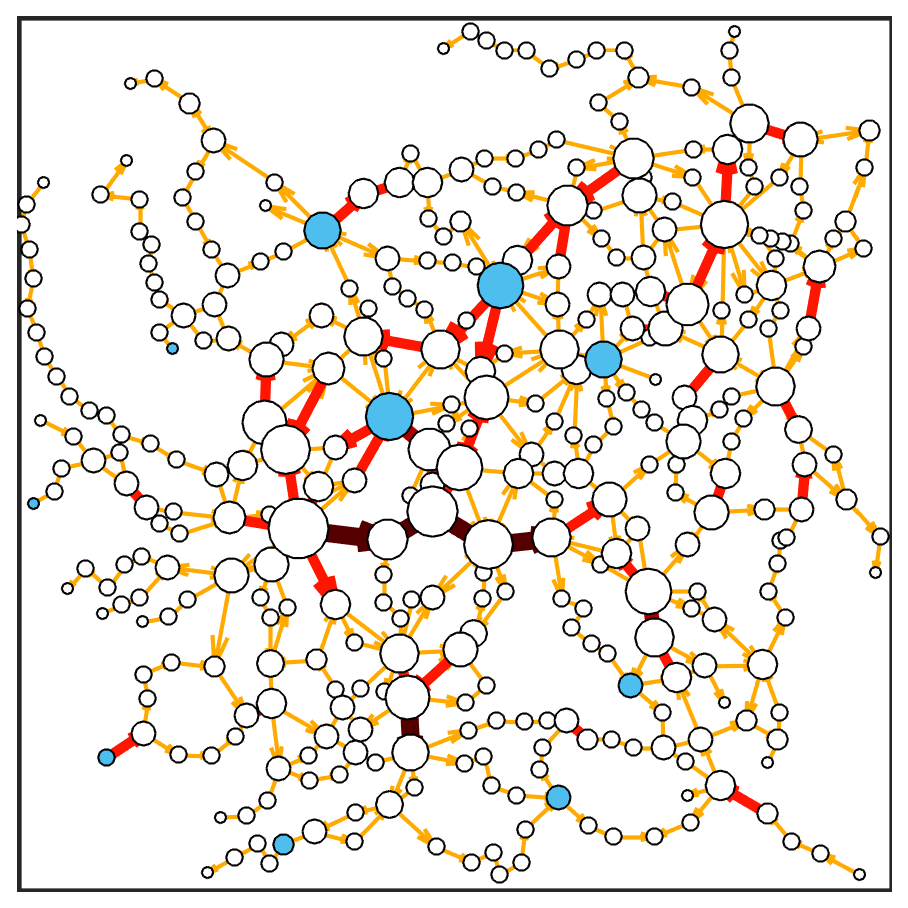
\includegraphics[width=48mm]{pics/syn2.eps}&
\includegraphics[width=48mm]{pics/syn3.eps}\\
(a) & (b) & (c) \\
\end{tabular}
% \vspace{-4mm}
\caption{
人工数据集和结果的示意图。(a)关键点和原始轨迹数据。10个五边形是随机生成的关键点。(b)多层次ROI网络的底层。蓝色ROI是关键ROI,其至少包含一个关键点。(c)轨迹检索结果。黑色轨迹是目标。检索结果为不同色调的绿色轨迹。颜色越深,与目标越相似,即包含更多关键ROI。}
\label{fig:syn}
% \vspace{-3mm}
\end{figure}


\smallsection{评价指标}
为了衡量语义检索结果的准确性,我们需要定义ROI和轨迹的真实目标。在人工实验中,真的关键节点隐含在10个关键点里。对于相似ROI检索任务,给定任何关键点,最相似的ROI应该是包含其他九个关键点的ROI,这些关键点被称为真实ROI。检索性能通过正确检测到的真实ROI的比率来衡量。对于轨迹检索任务,我们选择目标轨迹作为尽可能多地通过真实ROI。在这种情况中,目标轨迹应该包含尽可能多的真实ROI。因此,我们可以获得检索到的轨迹并进行排序,然后比较真实顺序和检索顺序来计算累计收益(NDCG@k),其定义如下。

接下来,我们可以执行ROI或者轨迹的语义检索了,并计算检索结果的ROI或者轨迹和真实ROI或轨迹之间的NDCG@k度量。此外,我们可以将算法的性能与国际最主流的相似性算法DTW,LCSS,EDR和Fr\'echet距离进行比较。在不失一般性的情况下,我们也在上述辅助ROI网络上计算这四个比较度量。
\begin{equation}
\mathrm{NDCG@k} = \frac{\mathrm{DCG@k}}{\mathrm{IDCG@k}},
\label{eq:NDCG}
\end{equation}
其中$\mathrm{IDCG@k}$是$\mathrm{DCG@k}$的理想取值,而$\mathrm{DCG@k}$定义如下:
\begin{equation}
\mathrm{DCG@{k}} = \sum_{i=1}^{k} \frac{ 2^{rel_{i}} - 1 }{ \log_{2}(i+1)},
\label{eq:DCG}
\end{equation}
其中$rel_i$是位置$i$处的相关度。为了试验更加清晰,我们采用5个级别的相关度。

\tabcolsep=0.5pt
% \vspace{-4mm}
\begin{figure}[!b]
% \vspace{-3mm}
\centering
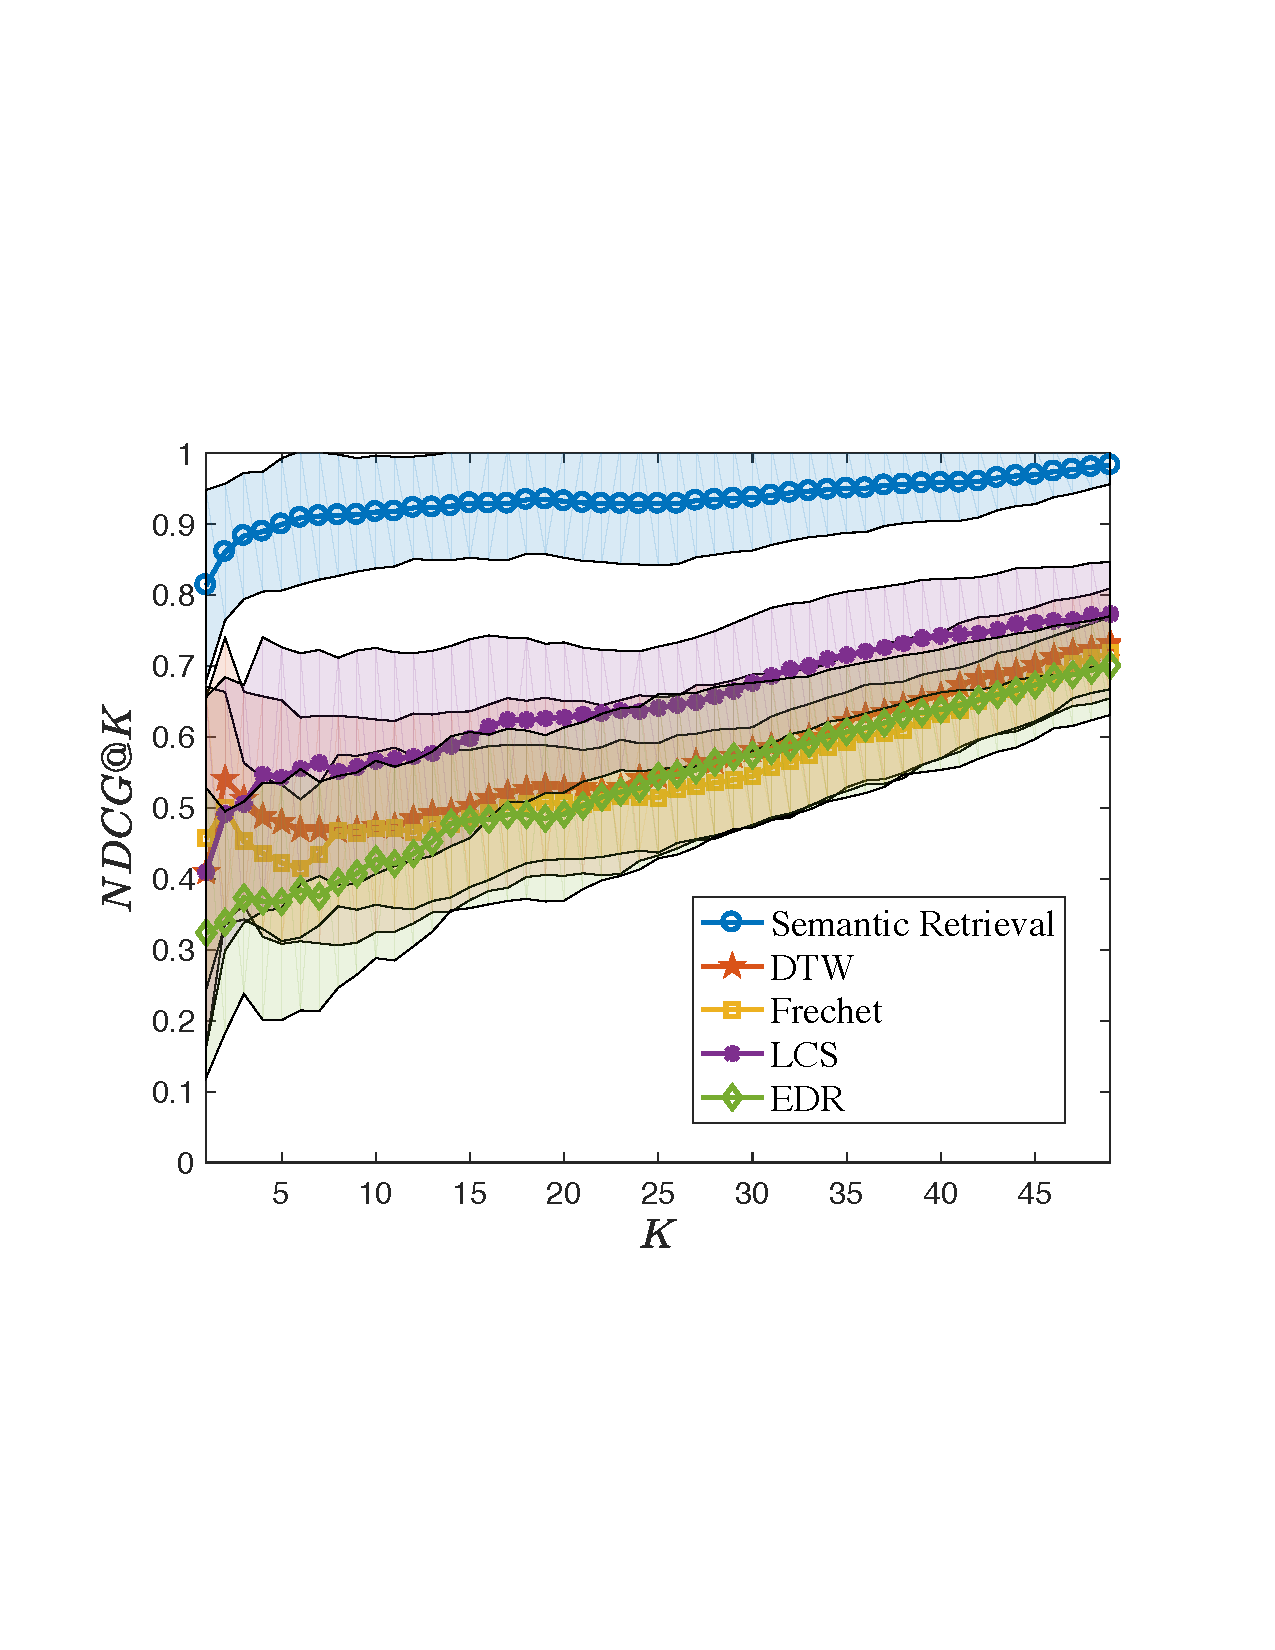
\includegraphics[width=100mm]{pics/synNDCG.pdf}
% \vspace{-4mm}
\caption{人工数据集上的语义轨迹检索结果。阴影部分是100次检索的标准差区域。}
\label{fig:synNDCG}
\end{figure}


\subsection{实验结果与分析}
% \subsection{人工数据集上的验证}
在人工数据集上设定交互范围 $\epsilon = \{2,4,6,8,10\}(m)$,运用\CascadeSync算法后得到一个5层的ROI网络。最下面的一层可视化在图\ref{fig:syn}(b)中。


\smallsection{人工数据集上的关键节点检测结果}
在此任务中,我们使用领域知识:ROI是否包含任何关键点。为了测试这些关键ROI是否具有相似的向量表征,我们评估了给定关键ROI的最相似ROI的检索准确性(图\ref{fig:syn}(b)中的蓝色ROI)。 理想的检索结果是所有关键ROI都比那些非关键ROI更相似。

在ROI和轨迹的嵌入向量的基础上,我们搜索最相似的ROI。实验在随机生成的数据集上独立重复100次。得到的平均准确度为$\boldsymbol{99.64\%}$,这证明了关键点的语义成功地整合到嵌入表示中,并且可以有效地检测到关键点。



\tabcolsep=2pt
\begin{figure}[!t]
\centering
% \vspace{-2mm}
% \footnotesize
\begin{tabular}{cc}
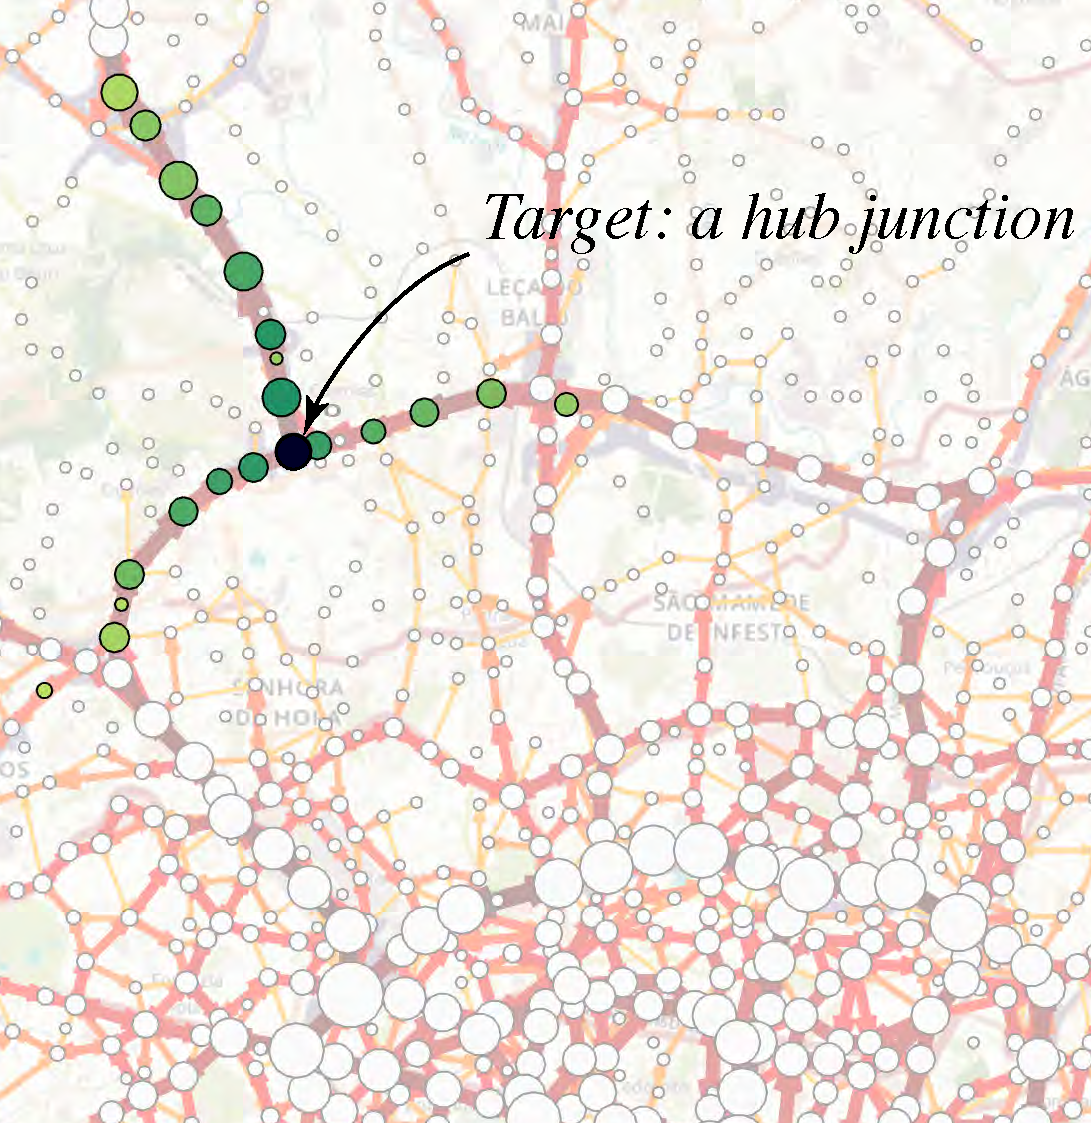
\includegraphics[width=65mm]{pics/SP3.pdf}&
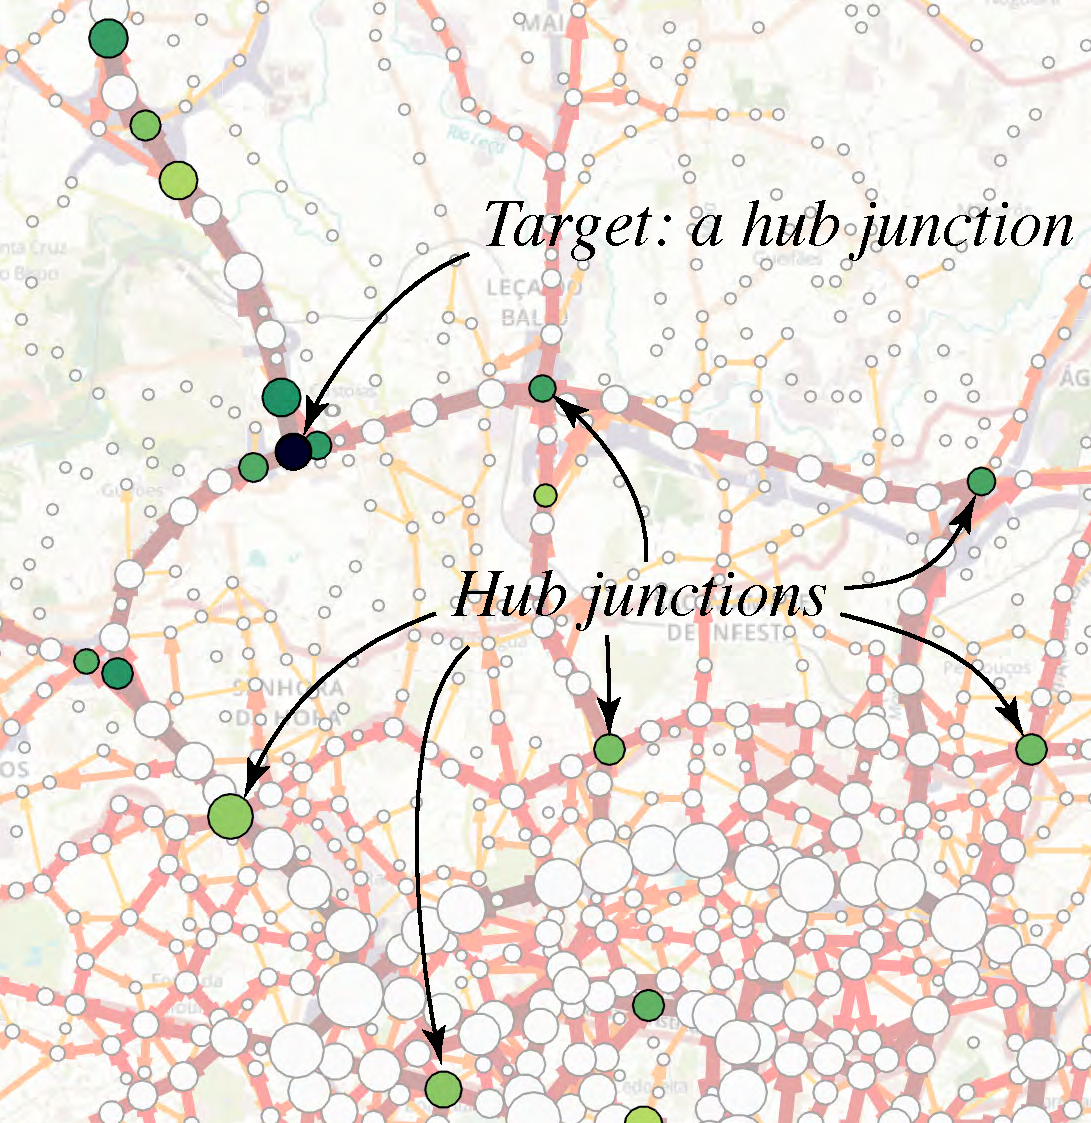
\includegraphics[width=65mm]{pics/SP4.pdf}\\
(a) 没有语义信息 & (b) 有语义信息
% \multicolumn{2}{c}{(a) Geolife} & & \multicolumn{2}{c}{(b) Kaggle Taxi}\\
\end{tabular}
% \vspace{-2mm}
\caption{在Kaggle数据集上的相似ROI检索结果。}
% \vspace{-2mm}
\label{fig:regionSim}
\end{figure}

\smallsection{人工数据集上的语义轨迹检测结果。}
我们在轨迹层面上进行类似的实验,目的是检索与包含最多关键ROI相似的目标轨迹,因此类似的轨迹应包含尽可能多的关键ROI。我们计算并确定其余49个轨迹与目标的相似度,并使用NDCG@k,即式(\ref{eq:NDCG})来给定排名。在图\ref{fig:syn}(c)中我们可视化了最相似的轨迹,其中绿色轨迹的颜色深浅与检索顺序成正比。此外,我们使用第一层ROI网络(具有关键ROI标签的最佳级别)上的四个对比算法进行相同的实验。结果如图\ref{fig:synNDCG}所示。实验重复100次,阴影部分给出平均NDCG@k值的标准偏差。从图中可以看出,我们的模型优于其他四个模型,很好地捕获了语义信息。




\smallsection{真实数据集上的检索结果}

实验的目标为给定一个ROI,检索前5个最相似的ROI,并计算NCDG@5。此外,给定一条轨迹,我们检索前10个最相似的轨迹,计算NCDG@3,5,10,并与对比算法进行比较。此外,我们将每个ROI邻居的数量设置为3,将负抽样的样本数设置为5,并交互范围设置为$\epsilon(l) = l \times 1/200\times(width + height), l = \{1,\cdots,5\}$来产生一个5层的ROI网络。

为了探索不同语义信息对现实数据检索性能的影响,我们取三种不同累心的模型来做实验:1)仅几何信息(即基本轨迹结构)。2)几何和基本语义(即网络特征和时间信息)。3)所有类型的邻居和领域知识。此外,我们通过构建两个嵌入模型来研究特征传播的效果:仅在ROI网络的底层($\epsilon(t) = 1/200 \times(width + height)$)用公式(\ref{eq:optimizeFun})进行训练,以及在ROI网络的5个层用式(\ref{eq:optimizeFunAll})进行训练。

为了更好地说明ROI检索的结果,我们选择Kaggle数据集中的一个枢纽十字路口作为目标ROI。我们在上述5层网络中运用了具有和不具有语义邻居的嵌入模型,检索结果如图\ref{fig:regionSim}所示。从结果来看,具有语义邻居的模型可以捕获语义信息,从而容易地识别区域的功能,并且能够检索到远离查询目标十字路口的其他枢纽十字路口。原因在于交通的语义可以通过节点度以及度分布的信息在ROI网络上反映出来,因此不会受到几何位置的限制。

ROI检索和轨迹检索的结果分别列在表\ref{tab:ROIEvaluation}和表\ref{tab:Evaluation_trajectory}中。从表中我们有三个发现:(1)嵌入模型中考虑的语义邻居越多,嵌入模型的性能越好;(2)当没有领域知识可用时,分层ROI网络上的嵌入模型优于单层模型的结果,这意味着分层结构通过特征传播促进了嵌入向量的表征能力。(3)当嵌入模型中融入领域知识后,性能主要依赖于领域知识的标签质量。


\tabcolsep=3pt
\begin{table}[tbh!]\renewcommand{\arraystretch}{1.3}
\caption{ROI检索在NDCG@5指标上的结果。模型1仅考虑几何邻居。模型2考虑了几何邻居和基本的语义信息。模型3考虑了真实的标签信息。}
% \vspace{-2mm}
\center
\small
\begin{tabular}{cccccc}
\hlinew{1pt}
\textbf{数据集} &\textbf{结构} & \textbf{Random} & \textbf{模型1} & \textbf{模型2}&\textbf{模型3} \\[0.4ex] \hlinew{0.85pt}
%Colon
\multirow{2}{*}{Geolife} & One-layer & \multirow{2}{*}{0.429 $\pm$ 0.24} & 0.526 $\pm$ 0.18 & 0.560 $\pm$ 0.15 & 0.713 $\pm$ 0.18\\
&Hierarchical & & 0.581 $\pm$ 0.15 & 0.615 $\pm$ 0.13 & \textbf{0.724 $\pm$ 0.17}\\
\hline
\multirow{2}{*}{T-Drive} & One-layer & \multirow{2}{*}{0.382 $\pm$ 0.23} & 0.592 $\pm$ 0.21 & 0.521 $\pm$ 0.18 & \textbf{0.713 $\pm$ 0.21}\\
&Hierarchical & & 0.650 $\pm$ 0.24 & 0.655 $\pm$ 0.23 & 0.693 $\pm$ 0.18\\
\hline
\multirow{2}{*}{Kaggle} & One-layer & \multirow{2}{*}{0.410 $\pm$ 0.28} & 0.524 $\pm$ 0.20 & 0.542 $\pm$ 0.22 & 0.679 $\pm$ 0.19\\
&Hierarchical & & 0.524 $\pm$ 0.22 & 0.567 $\pm$ 0.21 & \textbf{0.691 $\pm$ 0.16}\\
\hline
\multirow{2}{*}{Chengdu} & One-layer & \multirow{2}{*}{0.415 $\pm$ 0.25} & 0.666 $\pm$ 0.20 & 0.677 $\pm$ 0.21 & \textbf{0.817 $\pm$ 0.17}\\
&Hierarchical & & 0.697 $\pm$ 0.23 & 0.665 $\pm$ 0.20 & 0.802 $\pm$ 0.16\\
\hlinew{1pt}
\end{tabular}
\label{tab:ROIEvaluation}
\end{table}



\begin{table*}[tbh!]\renewcommand{\arraystretch}{1.3}
\caption{四个真实数据集上的轨迹语义检索。}
% \vspace{1mm}
\center
\small
\tabcolsep=2pt
\begin{tabular}{ccccccc}
\hlinew{1pt}
\textbf{数据集} & \textbf{指标} & \textbf{Random} & \textbf{DTW} & \textbf{Frechet} & \textbf{LCSS} & \textbf{EDR}\\
\hlinew{0.85pt}

\multirow{3}{*}{\textbf{Geolife}} 
&NDCG@3 &0.254 $\pm$ 0.158 & 0.391 $\pm$ 0.198 & 0.328$ \pm $0.179 & 0.360 $\pm$ 0.258 & 0.340 $\pm$ 0.189   \\
&NDCG@5 &0.272 $\pm$ 0.130 & 0.410 $\pm$ 0.185 & 0.393$ \pm $0.178 & 0.368 $\pm$ 0.224 & 0.411 $\pm$ 0.171   \\
&NDCG@10 &0.293 $\pm$ 0.127 & 0.521 $\pm$ 0.134 & 0.439$ \pm $0.165 & 0.379 $\pm$ 0.184 & 0.467 $\pm$ 0.171 \\
\hline
\multirow{3}{*}{\textbf{T-Drive}} 
&NDCG@3 &0.286 $\pm$ 0.182 & 0.416 $\pm$ 0.201 & 0.304$ \pm $0.191 & 0.396 $\pm$ 0.241 & 0.358 $\pm$ 0.195   \\
&NDCG@5 &0.290 $\pm$ 0.172 & 0.430 $\pm$ 0.168 & 0.346$ \pm $0.156 & 0.402 $\pm$ 0.211 & 0.363 $\pm$ 0.184   \\
&NDCG@10 &0.343 $\pm$ 0.169 & 0.443 $\pm$ 0.149 & 0.371$ \pm $0.141 & 0.402 $\pm$ 0.180 & 0.379 $\pm$ 0.161 \\
\hline
\multirow{3}{*}{\textbf{Kaggle}} 
&NDCG@3 &0.255 $\pm$ 0.220 & 0.311 $\pm$ 0.223 & 0.250$ \pm $0.175 & 0.349 $\pm$ 0.227 & 0.290 $\pm$ 0.182   \\
&NDCG@5 &0.276 $\pm$ 0.225 & 0.321 $\pm$ 0.215 & 0.288$ \pm $0.151 & 0.375 $\pm$ 0.218 & 0.304 $\pm$ 0.177   \\
&NDCG@10 &0.307 $\pm$ 0.201 & 0.342 $\pm$ 0.207 & 0.300$ \pm $0.148 & 0.382 $\pm$ 0.214 & 0.308 $\pm$ 0.162 \\
\hline
\multirow{3}{*}{\textbf{Chengdu}} 
&NDCG@3 &0.303 $\pm$ 0.210 & 0.417 $\pm$ 0.168 & 0.360$ \pm $0.239 & 0.314 $\pm$ 0.241 & 0.416 $\pm$ 0.196   \\
&NDCG@5 &0.320 $\pm$ 0.208 & 0.442 $\pm$ 0.153 & 0.388$ \pm $0.229 & 0.346 $\pm$ 0.221 & 0.424 $\pm$ 0.171   \\
&NDCG@10 &0.345 $\pm$ 0.205 & 0.457 $\pm$ 0.145 & 0.417$ \pm $0.211 & 0.376 $\pm$ 0.209 & 0.449 $\pm$ 0.179 \\
% \hlinew{1pt}
\end{tabular}

\tabcolsep=7pt
\begin{tabular}{ccccccc}
\hlinew{1pt}
\multirow{2}{*}{\textbf{数据集}} & \multirow{2}{*}{\textbf{指标}} & \multicolumn{2}{c}{\textbf{单层模型}} & \multicolumn{2}{c}{\textbf{多层模型}}\\
\cline{3-6}
&& \textbf{无领域知识} & \textbf{有领域知识} & \textbf{无领域知识} & \textbf{有领域知识}\\
\hlinew{0.85pt}

\multirow{3}{*}{\textbf{Geolife}} 
&NDCG@3 & 0.468 $\pm$ 0.177 & 0.607 $\pm$ 0.152 & 0.545 $\pm$ 0.171 & \textbf{0.663 $\pm$ 0.148} \\
&NDCG@5 & 0.483 $\pm$ 0.165 & 0.639 $\pm$ 0.120 & 0.552 $\pm$ 0.162 & \textbf{0.676 $\pm$ 0.104} \\
&NDCG@10& 0.520 $\pm$ 0.156 & 0.657 $\pm$ 0.109 & 0.558 $\pm$ 0.148 & \textbf{0.689 $\pm$ 0.094}\\
\hline
\multirow{3}{*}{\textbf{T-Drive}}
&NDCG@3 & 0.529 $\pm$ 0.169 & 0.697 $\pm$ 0.179 & 0.547 $\pm$ 0.182 & \textbf{0.717 $\pm$ 0.184} \\
&NDCG@5 & 0.545 $\pm$ 0.144 & \textbf{0.711 $\pm$ 0.172} & 0.564 $\pm$ 0.169 & 0.702 $\pm$ 0.183 \\
&NDCG@10& 0.544 $\pm$ 0.139 & \textbf{0.734 $\pm$ 0.168} & 0.599 $\pm$ 0.155 & 0.721 $\pm$ 0.175\\
\hline
\multirow{3}{*}{\textbf{Kaggle}}
&NDCG@3 & 0.406 $\pm$ 0.185 & 0.593 $\pm$ 0.164 & 0.438 $\pm$ 0.183 & \textbf{0.600 $\pm$ 0.209}\\
&NDCG@5 & 0.413 $\pm$ 0.160 & \textbf{0.604 $\pm$ 0.150} & 0.445 $\pm$ 0.151 & 0.602 $\pm$ 0.183\\
&NDCG@10& 0.430 $\pm$ 0.150 & 0.607 $\pm$ 0.157 & 0.452 $\pm$ 0.145 & \textbf{0.626 $\pm $0.188}\\
\hline
\multirow{3}{*}{\textbf{Chengdu}}
&NDCG@3 & 0.588 $\pm$ 0.159 & 0.824 $\pm$ 0.143 & 0.611 $\pm$ 0.160 & \textbf{0.833 $\pm$ 0.120}\\
&NDCG@5 & 0.622 $\pm$ 0.124 & \textbf{0.859 $\pm$ 0.139} & 0.635 $\pm$ 0.139 & 0.849 $\pm$ 0.112\\
&NDCG@10& 0.651 $\pm$ 0.112 & \textbf{0.866 $\pm$ 0.113} & 0.666 $\pm$ 0.114 & 0.862 $\pm$ 0.096\\
\hlinew{1pt}
\end{tabular}
\label{tab:Evaluation_trajectory}
\end{table*}

\section{本章小结}
在本章中,我们提出了一种新的语义轨迹嵌入表征方法。首先,经过 \CascadeSync模型将原始轨迹先转换为多层次的ROI网络。在这个网络上,可以依靠几何,语义,时间等信息以及作为上下文找到嵌入模型中的两种类型的邻居,其次利用负采样算法,计算出每一层ROI和轨迹的分布式表征向量。得到这个向量后,课通过直接计算向量间的欧几里德距离来高效地执行语义检索任务。在人工数据集和现实数据集上,本文的方法有效地提取并表征了语义信息,效果超过了四种主流算法。

% \newpage\mbox{}\thispagestyle{empty}\newpage
